% Figure 5 (PDF Figure 4): Qualitative cases for SynAP-Fib (arm E, best test
% checkpoint).
% Cases selected by the supervisor (node B, 2026-09-05) from the prespecified
% candidate lists in tables/fig5ai_candidates.md; F3 and the failure case were
% delegated to the executor with a representativeness mandate.
% Generated by figures/make_fig5.py from frozen predictions, lesion attention,
% and the expert box annotations (FACTS.md 10.1 provenance; no patient
% identifiers printed).
\begin{figure*}[!t]
\centering
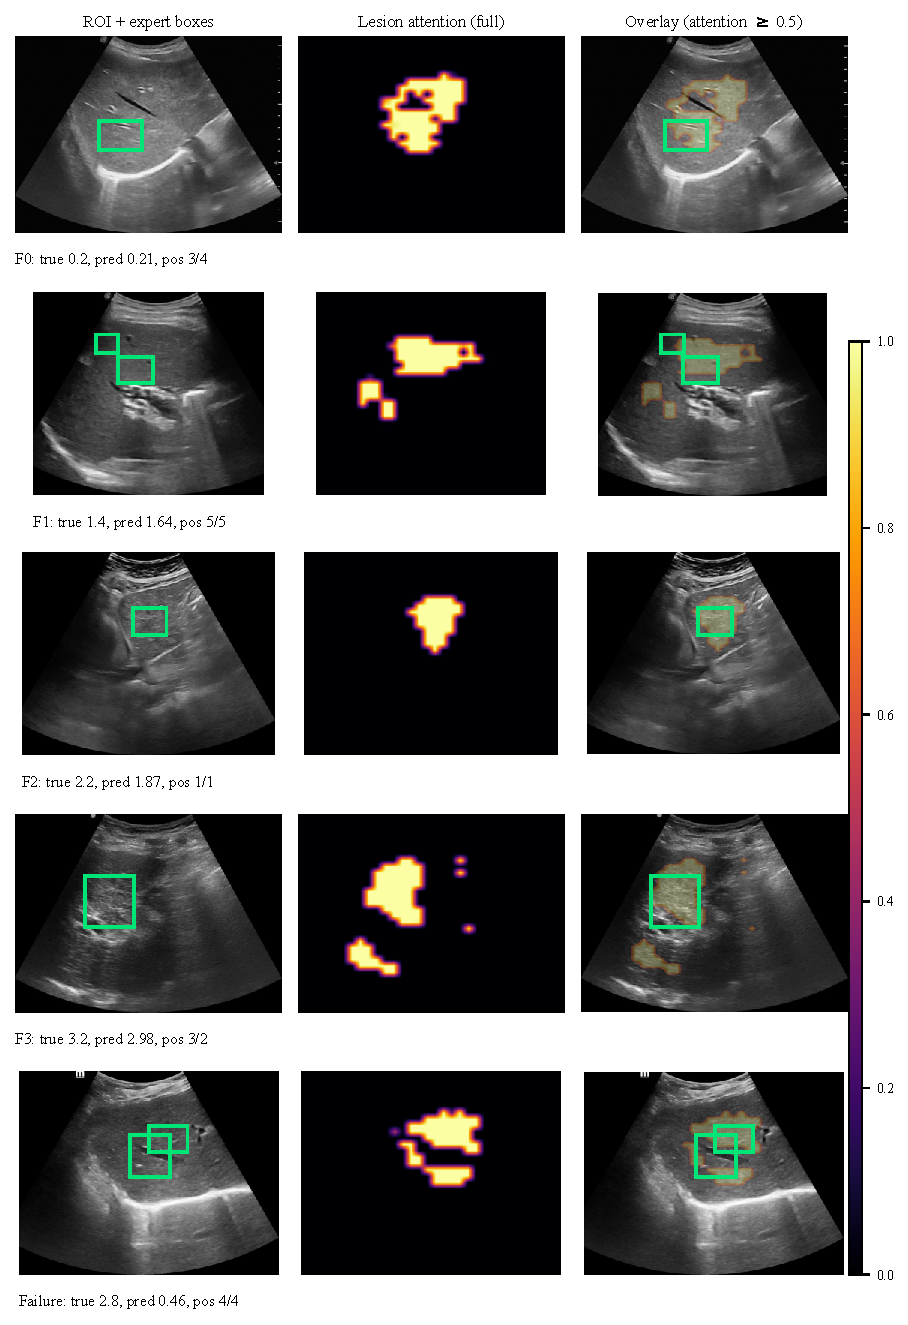
\includegraphics[width=0.98\textwidth]{figures/fig5_qualitative.pdf}
\caption{Qualitative results of the joint configuration (SynAP-Fib, arm E)
on the patient-held-out test set (seed 2026, validation-selected
checkpoint). Each row shows, from left to right: the original
region-of-interest image with the expert-annotated lesion boxes (green);
the complete predicted lesion attention map (upsampled from the
$32\times32$ head output, full $[0,1]$ range); and their overlay, in which
only attention at or above $0.5$ --- the binarization threshold used for
weak-box agreement --- is displayed together with the expert boxes. Rows
correspond to one representative case per clinical stage (top to bottom:
F0--F3) and one failure case with the largest prediction error in the test
set. For each row the annotation gives the true score, the predicted score,
and the true/predicted anatomical position (p1--p6). The attention maps are
weakly supervised and are shown as descriptive model behaviour; they are not
lesion segmentation ground truth, for which no pixel-level reference exists
in this cohort.}
\label{fig:qualitative}
\end{figure*}
